\begin{figure}
  \centering
  \def\W{1.5}
  \def\H{0.8}
  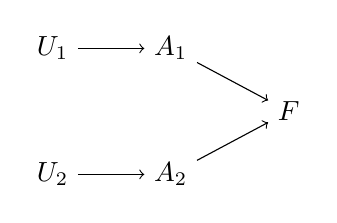
\begin{tikzpicture}
    \node (U1) at (   0, \H) {$U_1$};
    \node (U2) at (   0,-\H) {$U_2$};
    \node (A1) at (  \W, \H) {$A_1$};
    \node (A2) at (  \W,-\H) {$A_2$};
    \node (F)  at (2*\W,  0) {$F$};
    \draw[->] (U1) -- (A1);
    \draw[->] (U2) -- (A2);
    \draw[->] (A1) -- (F);
    \draw[->] (A2) -- (F);
  \end{tikzpicture}
  \caption{
    شبکه علّی برای مثال
    \ref{ex:causal-model}
  }
  \label{fig:cm-example-network}
\end{figure}
